\subsection{Overview}
{\label{sec:overview}}
\begin{figure*}
  \centering
  % Requires \usepackage{graphicx}
  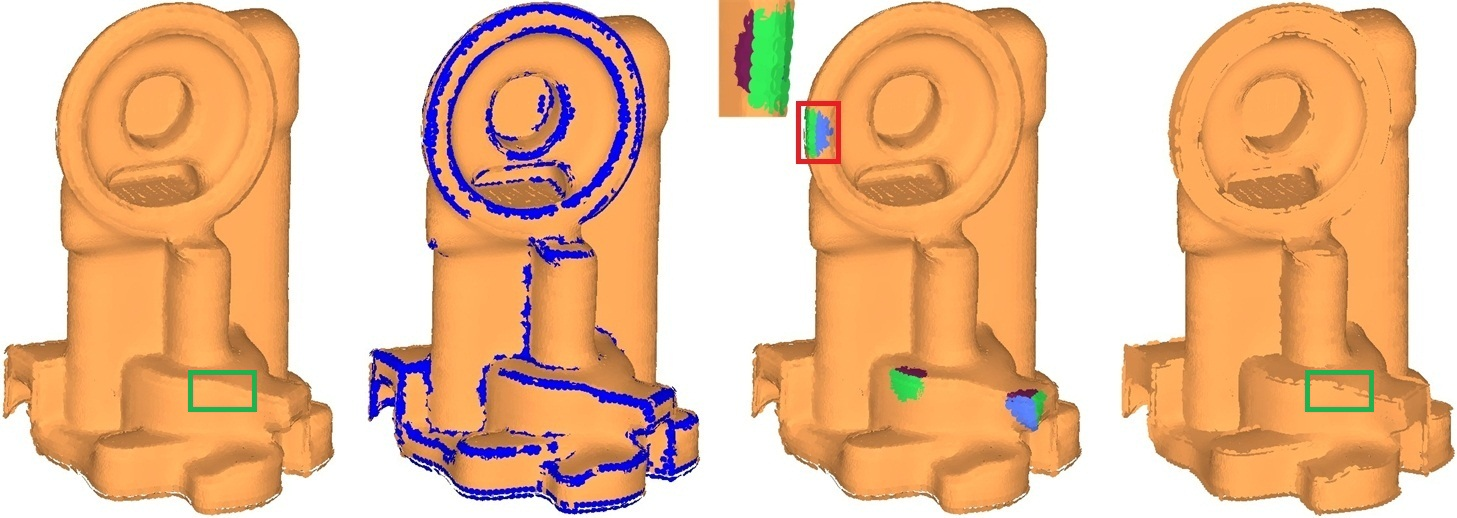
\includegraphics[width=0.8\linewidth]{oilpump_zj}\\
  \hspace{3 mm} (a) \hspace{28 mm} (b) \hspace{28 mm} (c)\hspace{28 mm} (d)
  \caption{Method overview.
         (a)Original model of oilpump. (b) Initial detected candidate feature points. (c)The classified subneighborhoods. (d)Estimated normals. }\label{fig:flow_chart}
\end{figure*}
With a noisy point cloud $\mathcal{P}=\{p_{i}\}_{i=1}^{N}$ as input, our algorithm takes three steps to estimate the normals preserving sharp features. First, we detect the points which are near the sharp features. Then, the neighborhoods of these points are segmented by their position and structure. Finally, using the results of segmentation we can select an anisotropic neighborhood to estimate the normal. The overall procedure of our method is shown in Fig. \ref{fig:flow_chart}.

\textbf{Candidate Feature Points Selection.} Normal estimation is challenging in the presence of sharp features. Hence we begin our method with a selection of points which are near sharp features and name them as \emph{candidate feature point}. Using covariance analysis of local neighborhoods, a weight is assigned to each vertex, which measures the likelihood of a vertex belongs to features. Candidate feature point are extracted by eliminating the vertex with low salience weight.
%We define the threshold automatically. First, we compute
%a histogram capturing the distribution of the weight $w$. Then the
%threshold is defined as the horizontal ordinate where the frequency
%begins to have a slow decrease.

\textbf{Subneighborhood Segmentation.} When the point is near sharp features, a neighborhood including distance smooth patches is likely to be got. We perform subspace clustering inside
the neighborhood of every candidate feature point to identify these patches. All the points in a single cluster represent a smooth region. To robustly segment these intersecting patches, we
propose a novel subspace clustering method based on structural low
rank presentation guided by credible regions. Our scheme improve the clustering results by taking both the local information and subspace structure into consideration.

\textbf{Normal Estimation} The actual normal estimation applied to a point is
chosen according to the category of the point.  If a point is not belong to the candidate feature points, the whole neighborhood is used to estimate the normal of the point. Otherwise, we choose the nearest cluster generated by subneighborhood segmentation to estimate the normal. 